\documentclass[presentation]{beamer}
\usepackage[utf8x]{inputenc}
\usepackage{ucs}
\usepackage{amsmath,tabularx}
\usetheme{Warsaw}
% \usecolortheme{crane}
% \usefonttheme{structurebold}
\newcolumntype{C}{>{\centering\arraybackslash}X}
\linespread{1}

\usepackage{subfigure}

\setcounter{footnote}{0}

\title[Hidden Structure]{\sc{Text as Data: What you need to know}}
\author[NA]{Nelson Auner}
 %Prof. Matt Taddy\footnotemark \footnotetext[1]{Associate Professor of Econometrics and Statistics at Chicago Booth School of Business},
% Prof. Stephen Stigler\footnotemark \footnotetext[2]{Ernest DeWitt Burton Distinguished Service Professor at the Department of Statistics of the University of Chicago}



\institute[TGG]{Prepared for TGG}
\date[16.10.2014]{October 16, 2014}

\usepackage{amsmath,supertabular,tabularx,graphicx,amssymb,amsfonts}
\usepackage{natbib,rotating}
%\usepackage{default}
\newcolumntype{Z}{>{\centering\arraybackslash}X}%



\renewcommand{\t}{\ensuremath{\theta}}
\renewcommand{\a}{\ensuremath{\alpha}}
\renewcommand{\b}{\ensuremath{\beta}}
\newcommand{\g}{\ensuremath{\gamma}}
\newcommand{\E}{\mathsf{E}}
\renewcommand{\d}{\ensuremath{\delta}}
\newcommand{\e}{\ensuremath{\epsilon}}
\newcommand{\s}{\sigma}
% \renewcommand{\S}{\Sigma}
\newcommand{\from}{\ensuremath{\leftarrow}}
\newcommand{\bm}{\mathbf}
\renewcommand{\l}{\lambda}
\newcommand{\dint}{\int\displaylimits}
\newcommand{\bx}{\mathbf x}
\newcommand{\by}{\mathbf y}
\newcommand{\be}{\pmb\e}
\renewcommand{\k}{\kappa}
\newcommand{\m}{\mu}
\newcommand{\A}{\ensuremath{\mathcal{A}}}
\newcommand{\B}{\ensuremath{\mathcal{B}}}
\newcommand{\sT}{\mathrm{T}}
\newcommand{\diag}{\mathrm{diag}}
\newcommand{\Tr}{\mathrm{Tr}}
\newcommand{\cov}{\mathbb{C}\mathrm{ov}~}
\newcommand{\var}{\mathbb{V}\mathrm{ar}~}


\AtBeginSection[]  % "Beamer, do the following at the start of every section"
{
\begin{frame}<beamer> 
\frametitle{Outline} % make a frame titled "Outline"
\tableofcontents[currentsection]  % show TOC and highlight current section
\end{frame}
}


\setcounter{footnote}{0}
\begin{document}

\begin{frame}
  \titlepage
\end{frame}

%%%%%%%%%%%%%%%%%%%


\begin{frame}
\frametitle{A quick aside...}
\begin{center}
\pause

\includegraphics[height=.8\textheight]{Images/badcode.jpg}
\end{center}
\pause
\end{frame}


\section{Motivation}

\begin{frame}
\frametitle{Drowning in text}
\pause
\begin{center}
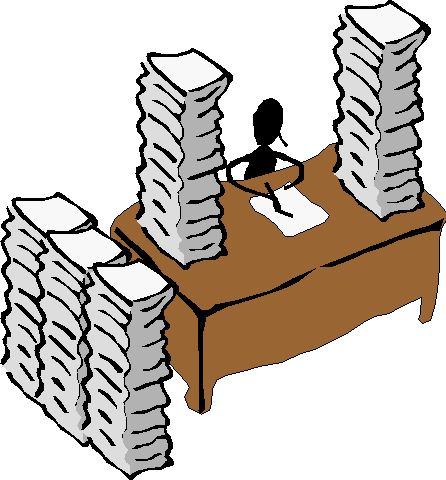
\includegraphics[height=.8\textheight]{Images/textdata.png}
\end{center}
\end{frame}

\begin{frame}
\frametitle{Motivation: Historical }
\pause
\begin{center}

\includegraphics[height=.8\textheight]{Images/federalist.jpg}
\end{center}
\end{frame}

\begin{frame}
\frametitle{Motivation: In the News}
\pause
\begin{center}
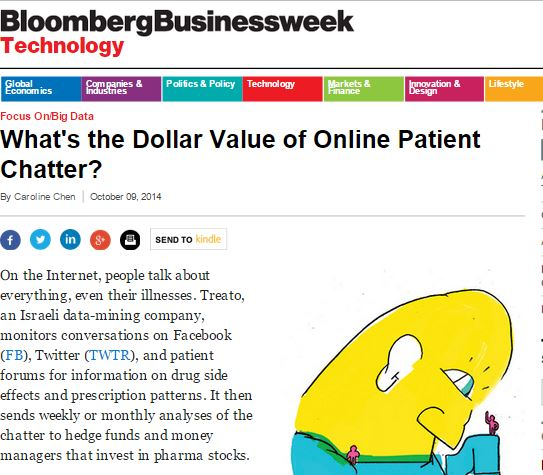
\includegraphics[height=.8\textheight]{Images/Treato.jpg}
\end{center}
\end{frame}

\begin{frame}
\frametitle{Public Sector Use}
\pause
\begin{center}
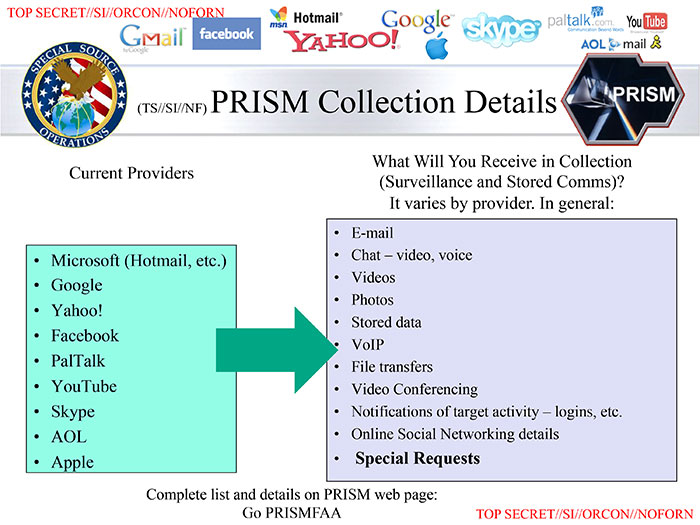
\includegraphics[height=.9\textheight]{Images/PRISM.jpg}
\end{center}
\end{frame}


\begin{frame}
\frametitle{How do they do it?}
\begin{itemize}
\pause
\item  "Treato distills the collective patient voice from blogs and forums using Natural Language Processing, Big Data and a proprietary patient language..."
%\item By the end of this talk, you should be able to guess at how treato works
\end{itemize}
\end{frame}

\section{Goals}


\begin{frame}
\frametitle{Are you comfortable talking about text?}
\pause
\begin{block}{Can you...}
\begin{itemize}
\pause
\item explain the basics of text analysis to a potential client?
\pause
\item identify opportunities to utilize text analysis?
\pause
\item commicate why text analysis is difficult?
\end{itemize}
\end{block}
\end{frame}



\section{Text as Data }
\subsection{Overview}
\begin{frame}
 \frametitle{The basics}
 \begin{itemize}
\pause
\item A document is a collection of words or phrases.
\pause
\item Our datasets are collections of documents
\end{itemize}
\pause
\begin{table}[!hbpt]
\caption{What did homework consist of? } \label{tab:title}
\pause
\begin{center}
\begin{tabular} {c c}
\textbf{Document} & \textbf{Content} \\
\hline
1 & Some computation and formula proving, a lot of R code \\
2 & Problems, computation using R \\
3 & Some computations and writing R code\\
4 & Proofs, problems, and programming work \\
\end{tabular}
\end{center}
\end{table}
\end{frame}

\subsection{Parsing}

\begin{frame}
\frametitle{Parsing}
\pause
\begin{itemize}
\item Greatest, Greatly, and Greatliest.... 
\pause
\end{itemize}
\begin{block}{It ain't that easy...}
\pause
Crystial rosey yeah I poe that \\
We connected with Cali we back door that \\
\pause
You see my wrist man keep your pink wrist bands \\ 
She can't believe I'm in a chevy even though I'm rich man \\
\pause
\textbf{Chevy Ridin' High - Dre (of Cool and Dre) f/ Rick Ross}
\end{block}
\end{frame}

\subsection{Multinomial Models}
\begin{frame}
\pause
\frametitle{Mo'(Multinomial) Models}
\begin{itemize}
\item If word order doesn't matter, then we can treat each document as a "bag of words". 
\pause
\item The number of words can be modeled $\sim$ multinomial
\pause
\end{itemize}
\begin{table}[!hbpt]
\caption{Creating a word-count matrix from text}
\begin{center} 
\resizebox{\textwidth}{!}{%
\begin{tabular}{ c |  c c c c c c c c c c c}
\hline
\textbf{Document} & Some & comp & formula & prov & R & code & use &
problem & writ & program & work \\
1 & 1 & 1 & 1 & 1 & 1 & 1 & 0 & 0 & 0 & 0 & 0 \\
2 & 0 & 1 & 0 & 0 & 1 & 0 & 1 & 1 & 0 & 0 & 0 \\
3 & 1 & 1 & 0 & 0 & 1 & 0 & 0 & 0 & 1 & 0 & 0\\
4 & 0 & 0 & 0 & 1 & 0 & 0 & 0 & 1 & 0 & 1 & 1\\
\hline
\end{tabular}}
\end{center}
\end{table} 
\end{frame}


\begin{frame}
\frametitle{A better model: Metadata}
\begin{itemize}
\item We would like to add structure to the model for inference or prediction
\pause
\item Metadata is data that accompanies a document
\pause
\end{itemize}
\begin{table}[!hbpt]
\caption{What did homework consist of?} \label{tab:title}
\pause
\begin{center}
\begin{tabular} {l l}
\textbf{Grade} & \textbf{Content} \\
\hline
A+ & Some computation and formula proving, a lot of R code \\
B & Problems, computation using R \\
B & Some computations and writing R code\\
C+ & Proofs, problems, and programming work \\  %something about R :P
\end{tabular}
\end{center}
\end{table}
\end{frame}

%\subsection{Metadata and Computation}
%\begin{frame}
%\frametitle{Metadata and Computation}
%\begin{itemize}
%\pause
%\item $n$ documents with metadata that takes $m$ discrete values:
%\pause
%\item Normally, $n >> m$
%\pause
%\item $\Rightarrow$ Collapse observations by outcome variables. 
%\pause
%\item Model as $m$ observations, instead of $n$
%\end{itemize}
%\pause
%\begin{table}[!hbpt]
%\begin{center}
%\resizebox{\textwidth}{!}{%
%\begin{tabular}{ l |  c c c c c c c c c c c}
%\hline
%\textbf{Document} & Some & comp & formula & prov & R & code & use &
%problem & writ & program & work \\
%A+ & 1 & 1 & 1 & 1 & 1 & 1 & 0 & 0 & 0 & 0 & 0 \\
%B & 1 & 2 & 0 & 0 & 2 & 0 & 1 & 1 & 1 & 0 & 0 \\
%C & 0 & 0 & 0 & 1 & 0 & 0 & 0 & 1 & 0 & 1 & 1\\
%\hline
%\end{tabular}}
%\end{center}
%\end{table} 
%\pause
%Reality: There are thousands of course reviews
%\end{frame}


\subsection{Topic Models}
\begin{frame}
 \frametitle{Topic Models}
A topic is a distribution of words. \\
In a topic model, documents are made of a mixtures of topics. 
\begin{columns}
\column{.3\textwidth}
\begin{block}<2->{Running Topic}
Stride, Pacing, Stretch
\end{block}
\column{.3\textwidth}
\begin{block}<3->{Bike Topic}
Pedal, Helmet, Gears
\end{block}
\column{.3\textwidth}
\begin{block}<4->{Swimming}
Stroke, Air, Water
\end{block}
\end{columns}
\begin{itemize}
\item<5-> A book about triathalon training $\sim$ $\theta_1$ Running + $\theta_2$ Biking + $\theta_3$ Swimming
\item<6-> Issue: We can no longer collapse observations, must use all $n$ observations
\item <7-> Workarounds: See Ryan's paper\footnotemark \footnotetext[1] {Wang, 2012. Sparse Coding and an Application to Topic Modeling.}
or mine \footnotemark \footnotetext[2]{Auner, 2014. Combining Latent Topics with Document Attributes in Text Analysis}
\end{itemize}
\end{frame}

\section{Applications}

\begin{frame}
\frametitle{Uncovering relationships}
\pause
\begin{center}
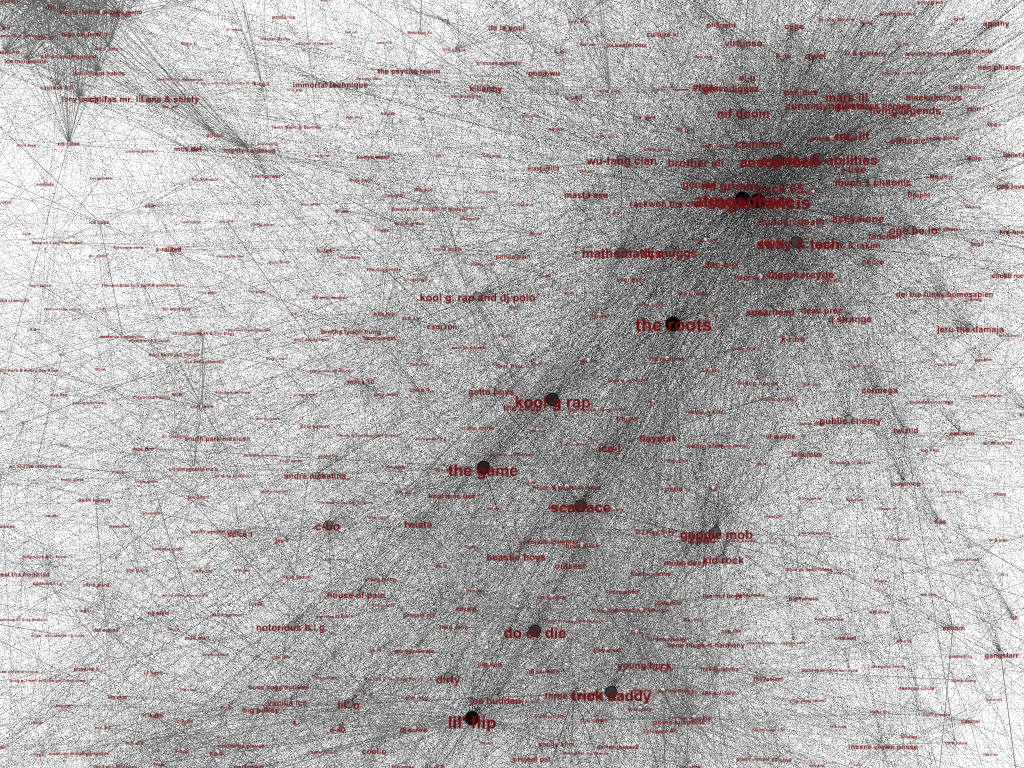
\includegraphics[height=.8\textheight]{Images/lyricsnetwork.png}
\end{center}
\end{frame}


\begin{frame}
\frametitle{Uncovering topics}
\begin{table}[!htbp]
\caption{Comparison of top word loadings on a stem-cell topic} \label{tab:title}
\centering
\begin{tabular}{  c  c }
Cluster Membership & Topic Model (LDA)* \\
\hline
umbilic.cord.blood & pluripotent.stem.cel \\
cord.blood.stem  & national.ad.campaign \\
blood.stem.cel   & cel.stem.cel \\
adult.stem.cel & stem.cel.line \\
\end{tabular}
\end{table}
\pause
*Results reported in Taddy (2012)
\end{frame}



\begin{frame}
\frametitle{Topics on Yelp} %Graph of first topic:
\begin{center}
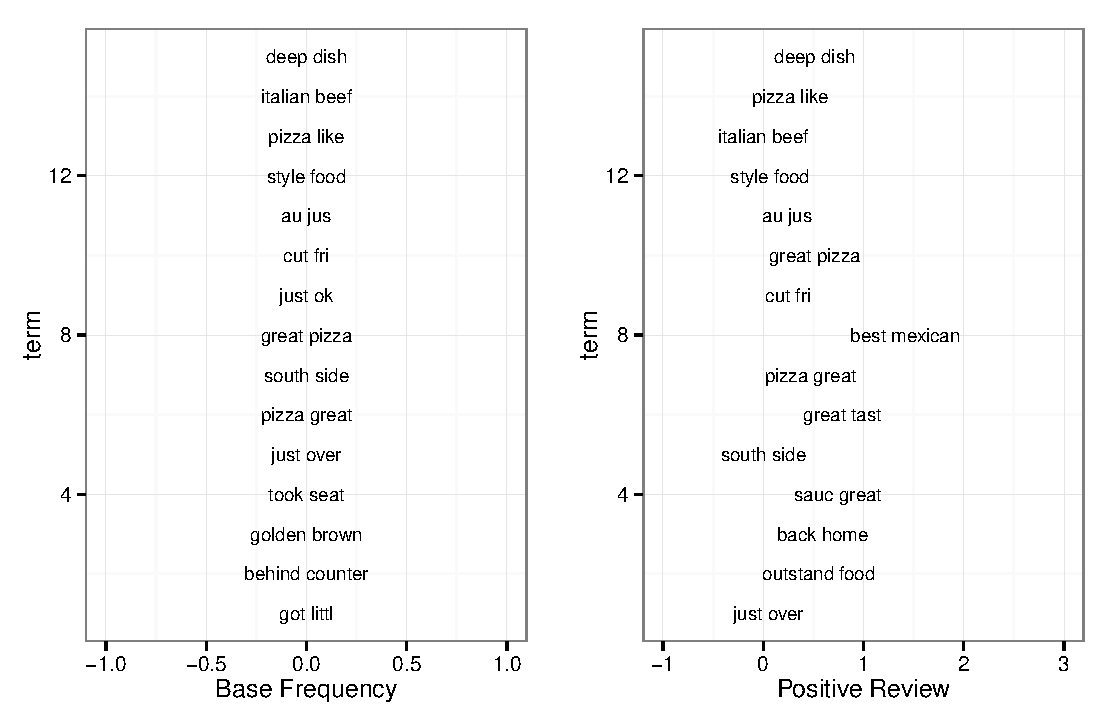
\includegraphics[width=1\textwidth]{Images/we8there_distortion.pdf}
\end{center}
\end{frame}


\begin{frame}
\frametitle{Imma Let you Finish, but the Dirichlet was the greatest prior of all time!}
\pause
\begin{center}
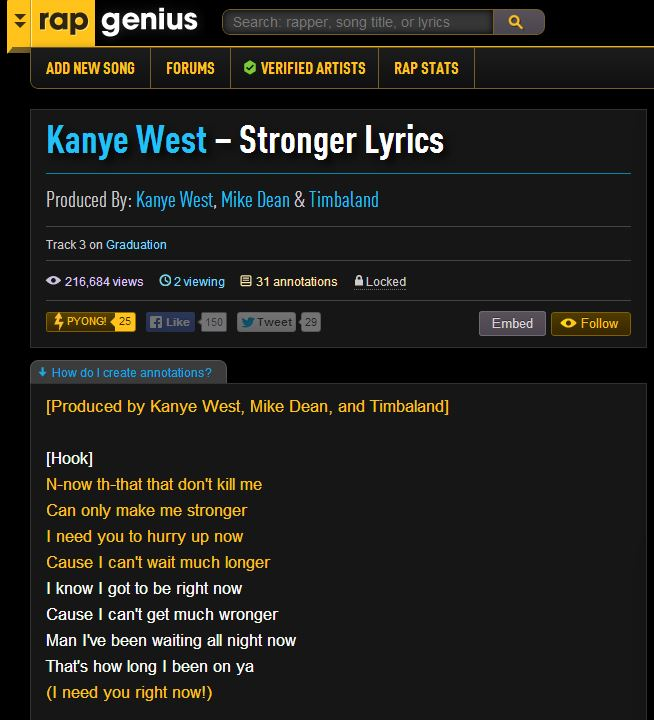
\includegraphics[height=1.0\textheight]{Images/lyrics_sample.png}
\end{center}
\end{frame}

\begin{frame} 	
\frametitle{Results}
\pause
% latex table generated in R 3.0.2 by xtable 1.7-1 package
% Mon May 12 22:33:48 2014
\begin{table}[ht]
\centering
\begin{tabular}{rll}
  \hline
 & term & loading \\ 
  \hline
1 & yeezus & 5.48 \\ 
  2 & constel & 3.79 \\ 
  3 & homm & 3.79 \\ 
  4 & preach & 3.79 \\ 
  5 & bound & 3.6 \\ 
  6 & thoma & 3.38 \\ 
  7 & thirti & 3.32 \\ 
  8 & rocka & 3.31 \\ 
  9 & rowland & 3.25 \\ 
  10 & jamaican & 3.23 \\ 
  11 & blocka & 3.22 \\ 
  12 & movement & 3.22 \\ 
  13 & unlik & 3.08 \\ 
  14 & yknow & 3.08 \\ 
   \hline
\end{tabular}
\end{table}
\end{frame}

\begin{frame}
\frametitle{Dip your feet in}
\pause
\begin{itemize}
\item \textit{Textir} or \textit{Gamlr} 
\item Currently only for R
\item Python coming soon!
\end{itemize}
\end{frame}

\begin{frame}
\frametitle{Thank You}
\begin{itemize}
\item Math: $ x_{i} \sim MN(q_{ij},m_{ij})    ; ~~  q_{ij} = \frac{exp(\alpha_j + y_i \phi_j + u_i \Gamma_{kj})}{\sum_{l=1}^{p}{exp(\alpha_l+ y_i \phi_l + u_i \Gamma_{kl})}} $
\item Talk based on \\ \textit{Combining Latent Topics with Document Attributes in Text Analysis}
\item Advisors: 
 Prof. Matt Taddy\footnotemark \footnotetext[2]{Associate Professor of Econometrics and Statistics at Chicago Booth School of Business},
Prof. Stephen Stigler\footnotemark \footnotetext[3]{Ernest DeWitt Burton Distinguished Service Professor at the Department of Statistics of the University of Chicago}
\end{itemize}
\end{frame}


\end{document}

